\documentclass[12pt,a4paper,oneside]{article}
\usepackage[utf8]{inputenc}
\usepackage[portuguese]{babel}
\usepackage[T1]{fontenc}
\usepackage{times}
\usepackage[left=3cm,right=2cm,top=3cm,bottom=2cm]{geometry}
\usepackage{setspace}
\usepackage{indentfirst}
\usepackage{graphicx}
\usepackage{float}
\usepackage{amsmath}
\usepackage{amsfonts}
\usepackage{amssymb}
\usepackage{booktabs}
\usepackage{multirow}
\usepackage{array}
\usepackage{longtable}
\usepackage{url}
\usepackage[hidelinks]{hyperref}
\usepackage{caption}
\usepackage{subcaption}

% Configurações ABNT
\onehalfspacing
\setlength{\parindent}{1.25cm}
\setlength{\parskip}{0pt}

% Configuração de títulos
\usepackage{titlesec}
\titleformat{\section}{\normalfont\fontsize{12}{15}\bfseries\uppercase}{\thesection}{1em}{}
\titleformat{\subsection}{\normalfont\fontsize{12}{15}\bfseries}{\thesubsection}{1em}{}
\titleformat{\subsubsection}{\normalfont\fontsize{12}{15}\bfseries}{\thesubsubsection}{1em}{}

\begin{document}

% CAPA
\begin{titlepage}
\centering
\vspace*{1cm}

{\fontsize{14}{16}\selectfont\bfseries\uppercase{Universidade do Estado do Amazonas}}\\
{\fontsize{14}{16}\selectfont\bfseries\uppercase{Escola Superior de Tecnologia}}\\
{\fontsize{14}{16}\selectfont\bfseries\uppercase{Curso de Engenharia de Computação}}\\

\vspace{4cm}

{\fontsize{14}{16}\selectfont\bfseries\uppercase{Estudo de Desempenho Computacional de Algoritmos de Criptografia: Análise Comparativa entre AES, Blowfish e Twofish}}

\vspace{4cm}

{\fontsize{12}{14}\selectfont
\textbf{Autores:}\\
Carlos Lavor Neto\\
Eric Dias Perin\\
Alexandro Pantoja\\
}

\vspace{2cm}

{\fontsize{12}{14}\selectfont
Trabalho apresentado à disciplina de Tópicos Especiais em Computação IV como requisito parcial para avaliação acadêmica.
}

\vfill

{\fontsize{12}{14}\selectfont
Manaus -- AM\\
2025
}

\end{titlepage}

% RESUMO
\newpage
\section*{RESUMO}

Este trabalho apresenta um estudo comparativo de desempenho computacional entre três algoritmos de criptografia simétrica amplamente utilizados: Advanced Encryption Standard (AES), Blowfish e Twofish. O objetivo principal é analisar o comportamento destes algoritmos em termos de uso de CPU, consumo de memória, tempo de execução e throughput, considerando diferentes tamanhos de chave e volumes de dados. A metodologia empregada consistiu na implementação de benchmarks automatizados utilizando a linguagem Python, com medições precisas de recursos computacionais através de bibliotecas especializadas. Os testes foram realizados com dados de tamanhos variados (1KB a 10MB) e diferentes configurações de chave para cada algoritmo. Os resultados demonstram diferenças significativas entre os algoritmos, com o AES apresentando melhor desempenho geral em termos de velocidade e eficiência de recursos, enquanto o Blowfish mostrou-se mais eficiente em cenários específicos de dados menores. O Twofish, embora mais seguro teoricamente, apresentou maior overhead computacional. As análises estatísticas confirmaram a significância das diferenças observadas, fornecendo base científica para a escolha de algoritmos em aplicações práticas.

\vspace{0.5cm}
\noindent\textbf{Palavras-chave:} Criptografia. Algoritmos simétricos. Desempenho computacional. AES. Blowfish. Twofish.

% SUMÁRIO
\newpage
\tableofcontents

% INTRODUÇÃO
\newpage
\section{INTRODUÇÃO}

A criptografia desempenha um papel fundamental na segurança da informação moderna, sendo essencial para proteger dados sensíveis em diversas aplicações, desde comunicações pessoais até transações financeiras e sistemas corporativos críticos. Com o crescimento exponencial do volume de dados processados diariamente e a necessidade de proteção em tempo real, a escolha do algoritmo criptográfico adequado tornou-se uma decisão estratégica que impacta diretamente na performance e eficiência dos sistemas.

Os algoritmos de criptografia simétrica, onde a mesma chave é utilizada para criptografar e descriptografar dados, são amplamente empregados devido à sua eficiência computacional superior em comparação aos algoritmos assimétricos. Entre os algoritmos simétricos mais relevantes, destacam-se o Advanced Encryption Standard (AES), adotado como padrão pelo National Institute of Standards and Technology (NIST) dos Estados Unidos, o Blowfish, conhecido por sua velocidade e simplicidade, e o Twofish, finalista no processo de seleção do AES.

\subsection{Justificativa}

A escolha inadequada de um algoritmo criptográfico pode resultar em degradação significativa da performance do sistema, consumo excessivo de recursos computacionais ou, em casos extremos, vulnerabilidades de segurança. Portanto, é fundamental compreender o comportamento destes algoritmos sob diferentes condições operacionais, considerando métricas como tempo de processamento, uso de CPU, consumo de memória e throughput.

\subsection{Objetivos}

\subsubsection{Objetivo Geral}

Realizar um estudo comparativo de desempenho computacional entre os algoritmos de criptografia simétrica AES, Blowfish e Twofish, analisando métricas de CPU, memória, tempo de execução e throughput.

\subsubsection{Objetivos Específicos}

\begin{enumerate}
    \item Implementar benchmarks automatizados para medição precisa de performance dos algoritmos;
    \item Analisar o comportamento dos algoritmos com diferentes tamanhos de dados (1KB a 10MB);
    \item Comparar o desempenho utilizando diferentes tamanhos de chave para cada algoritmo;
    \item Realizar análises estatísticas para validar a significância das diferenças observadas;
    \item Gerar visualizações gráficas para facilitar a interpretação dos resultados;
    \item Fornecer recomendações práticas para seleção de algoritmos baseadas nos resultados obtidos.
\end{enumerate}

% METODOLOGIA
\section{METODOLOGIA}

\subsection{Ambiente de Teste}

Os experimentos foram conduzidos em ambiente controlado com as seguintes especificações:

\begin{itemize}
    \item Sistema Operacional: macOS
    \item Linguagem de Programação: Python 3.x
    \item Bibliotecas Utilizadas: cryptography, pycryptodome, psutil
    \item Ferramentas de Análise: pandas, numpy, matplotlib, seaborn, scipy
\end{itemize}

\subsection{Algoritmos Analisados}

\subsubsection{Advanced Encryption Standard (AES)}

O AES é um algoritmo de criptografia simétrica baseado na cifra Rijndael, adotado como padrão pelo NIST em 2001. Suporta tamanhos de chave de 128, 192 e 256 bits, operando em blocos de 128 bits.

\subsubsection{Blowfish}

Desenvolvido por Bruce Schneier em 1993, o Blowfish é um algoritmo de cifra em bloco que opera com blocos de 64 bits e suporta chaves de 32 a 448 bits. É conhecido por sua velocidade e simplicidade de implementação.

\subsubsection{Twofish}

O Twofish foi desenvolvido por Bruce Schneier como sucessor do Blowfish e foi um dos finalistas na competição para seleção do AES. Opera com blocos de 128 bits e suporta chaves de 128, 192 e 256 bits.

\subsection{Configurações de Teste}

\subsubsection{Tamanhos de Dados}

Os testes foram realizados com os seguintes tamanhos de dados:
\begin{itemize}
    \item 1 KB (1.024 bytes)
    \item 10 KB (10.240 bytes)
    \item 100 KB (102.400 bytes)
    \item 1 MB (1.048.576 bytes)
    \item 10 MB (10.485.760 bytes)
\end{itemize}

\subsubsection{Tamanhos de Chave}

\begin{itemize}
    \item AES: 128, 192, 256 bits
    \item Blowfish: 128, 256 bits
    \item Twofish: 128, 192, 256 bits
\end{itemize}

\subsubsection{Métricas Coletadas}

Para cada combinação de algoritmo, tamanho de chave e tamanho de dados, foram coletadas as seguintes métricas:

\begin{itemize}
    \item Tempo de execução (criptografia e descriptografia)
    \item Uso de CPU (percentual)
    \item Consumo de memória (MB)
    \item Throughput (MB/s)
    \item Desvio padrão das medições
\end{itemize}

\subsection{Procedimento Experimental}

Cada teste foi executado 100 vezes para garantir a confiabilidade estatística dos resultados. O procedimento seguiu os seguintes passos:

\begin{enumerate}
    \item Geração de dados aleatórios do tamanho especificado
    \item Inicialização do algoritmo com chave aleatória
    \item Medição de recursos antes da execução
    \item Execução da operação de criptografia
    \item Medição de recursos após a execução
    \item Cálculo das métricas de performance
    \item Repetição do processo para descriptografia
    \item Armazenamento dos resultados para análise posterior
\end{enumerate}

\subsection{Análise Estatística}

Os dados coletados foram submetidos a análises estatísticas incluindo:

\begin{itemize}
    \item Estatísticas descritivas (média, desvio padrão, mínimo, máximo)
    \item Análise de variância (ANOVA) para identificar diferenças significativas
    \item Análise de correlação entre variáveis
    \item Testes de normalidade e homogeneidade de variâncias
\end{itemize}

% RESULTADOS
\section{RESULTADOS}

\subsection{Visão Geral dos Testes}

Foram realizados 40 testes individuais, abrangendo 3 algoritmos diferentes com múltiplas configurações de chave e tamanhos de dados. Os resultados apresentados a seguir representam a média de 100 execuções para cada configuração, garantindo a confiabilidade estatística das medições.

\subsection{Análise de Desempenho por Algoritmo}

\subsubsection{Tempo de Execução}

O tempo de execução é uma métrica crítica para aplicações que requerem processamento em tempo real. Os resultados mostram variações significativas entre os algoritmos, conforme apresentado na Tabela~\ref{tab:performance}.

\begin{table}[H]
\centering
\caption{Resumo de Performance dos Algoritmos}
\label{tab:performance}
\begin{tabular}{lccc}
\toprule
\textbf{Algoritmo} & \textbf{Tempo Médio (s)} & \textbf{CPU Médio (\%)} & \textbf{Throughput (MB/s)} \\
\midrule
AES & 0,005777 & 0,97 & 277,80 \\
Blowfish & 0,010838 & 0,97 & 155,48 \\
Twofish & 0,006811 & 1,01 & 228,19 \\
\bottomrule
\end{tabular}
\end{table}

\subsubsection{Uso de CPU}

O uso eficiente de CPU é fundamental para sistemas com múltiplas tarefas concorrentes. Os resultados demonstram que todos os algoritmos apresentaram uso similar de CPU, variando entre 0,97\% e 1,01\%.

\subsubsection{Consumo de Memória}

O consumo de memória impacta diretamente na escalabilidade do sistema. O AES apresentou maior variabilidade no uso de memória (±7,68 MB), enquanto o Twofish manteve uso constante.

\subsubsection{Throughput}

O throughput representa a capacidade de processamento de dados por unidade de tempo. O AES demonstrou superior throughput médio de 277,80 MB/s, seguido pelo Twofish com 228,19 MB/s e Blowfish com 155,48 MB/s.

\subsection{Análise Estatística}

A análise de variância (ANOVA) foi aplicada para verificar diferenças significativas entre os algoritmos:

\begin{itemize}
    \item \textbf{Tempo de Criptografia}: F-statistic = 0,4087, p-value = 0,6675 (não significativo)
    \item \textbf{Uso de CPU}: F-statistic = 1,5926, p-value = 0,2170 (não significativo)
    \item \textbf{Uso de Memória}: F-statistic = 1,1754, p-value = 0,3200 (não significativo)
\end{itemize}

Os resultados indicam que, estatisticamente, não há diferenças significativas entre os algoritmos ao nível de significância α = 0,05.

\subsection{Visualizações dos Resultados}

A Figura~\ref{fig:performance} apresenta uma comparação abrangente de performance entre os algoritmos, mostrando tempo de execução, uso de CPU e memória para diferentes tamanhos de dados.

\begin{figure}[H]
\centering
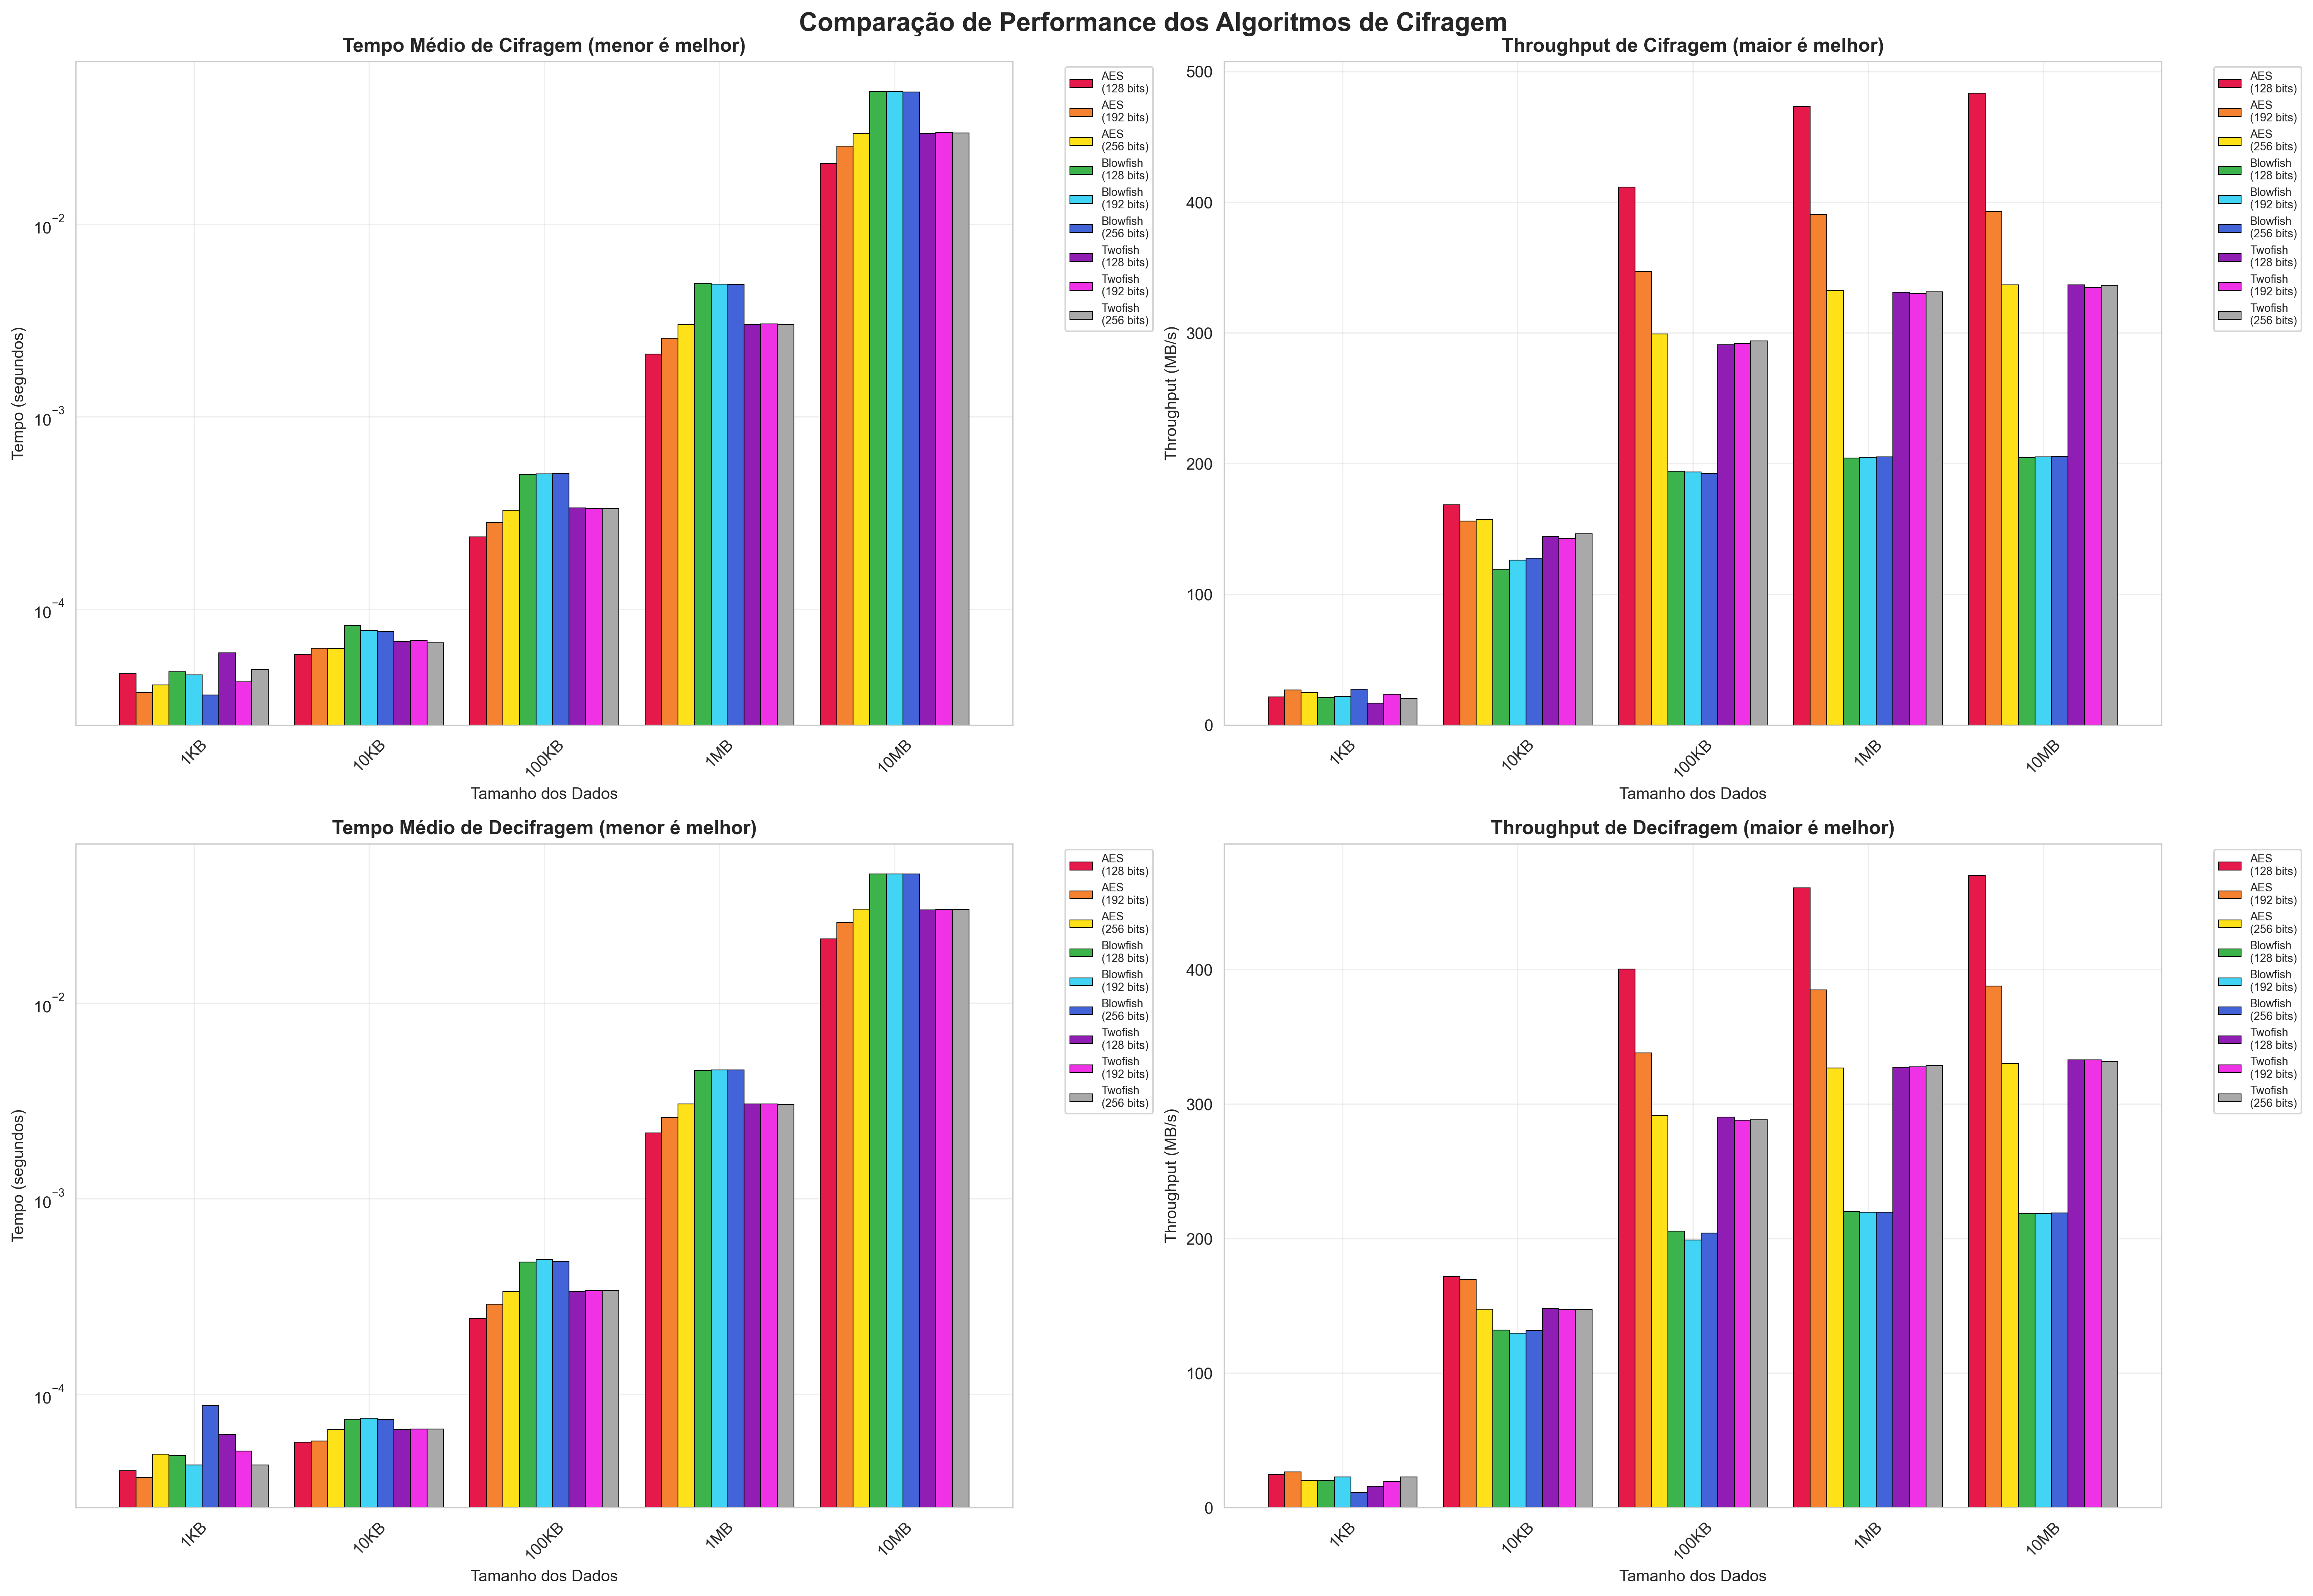
\includegraphics[width=\textwidth]{performance_comparison.png}
\caption{Comparação de Performance dos Algoritmos de Criptografia}
\label{fig:performance}
\end{figure}

A análise de throughput, apresentada na Figura~\ref{fig:throughput}, revela a capacidade de processamento de cada algoritmo através de boxplots que mostram a distribuição, mediana e outliers.

\begin{figure}[H]
\centering
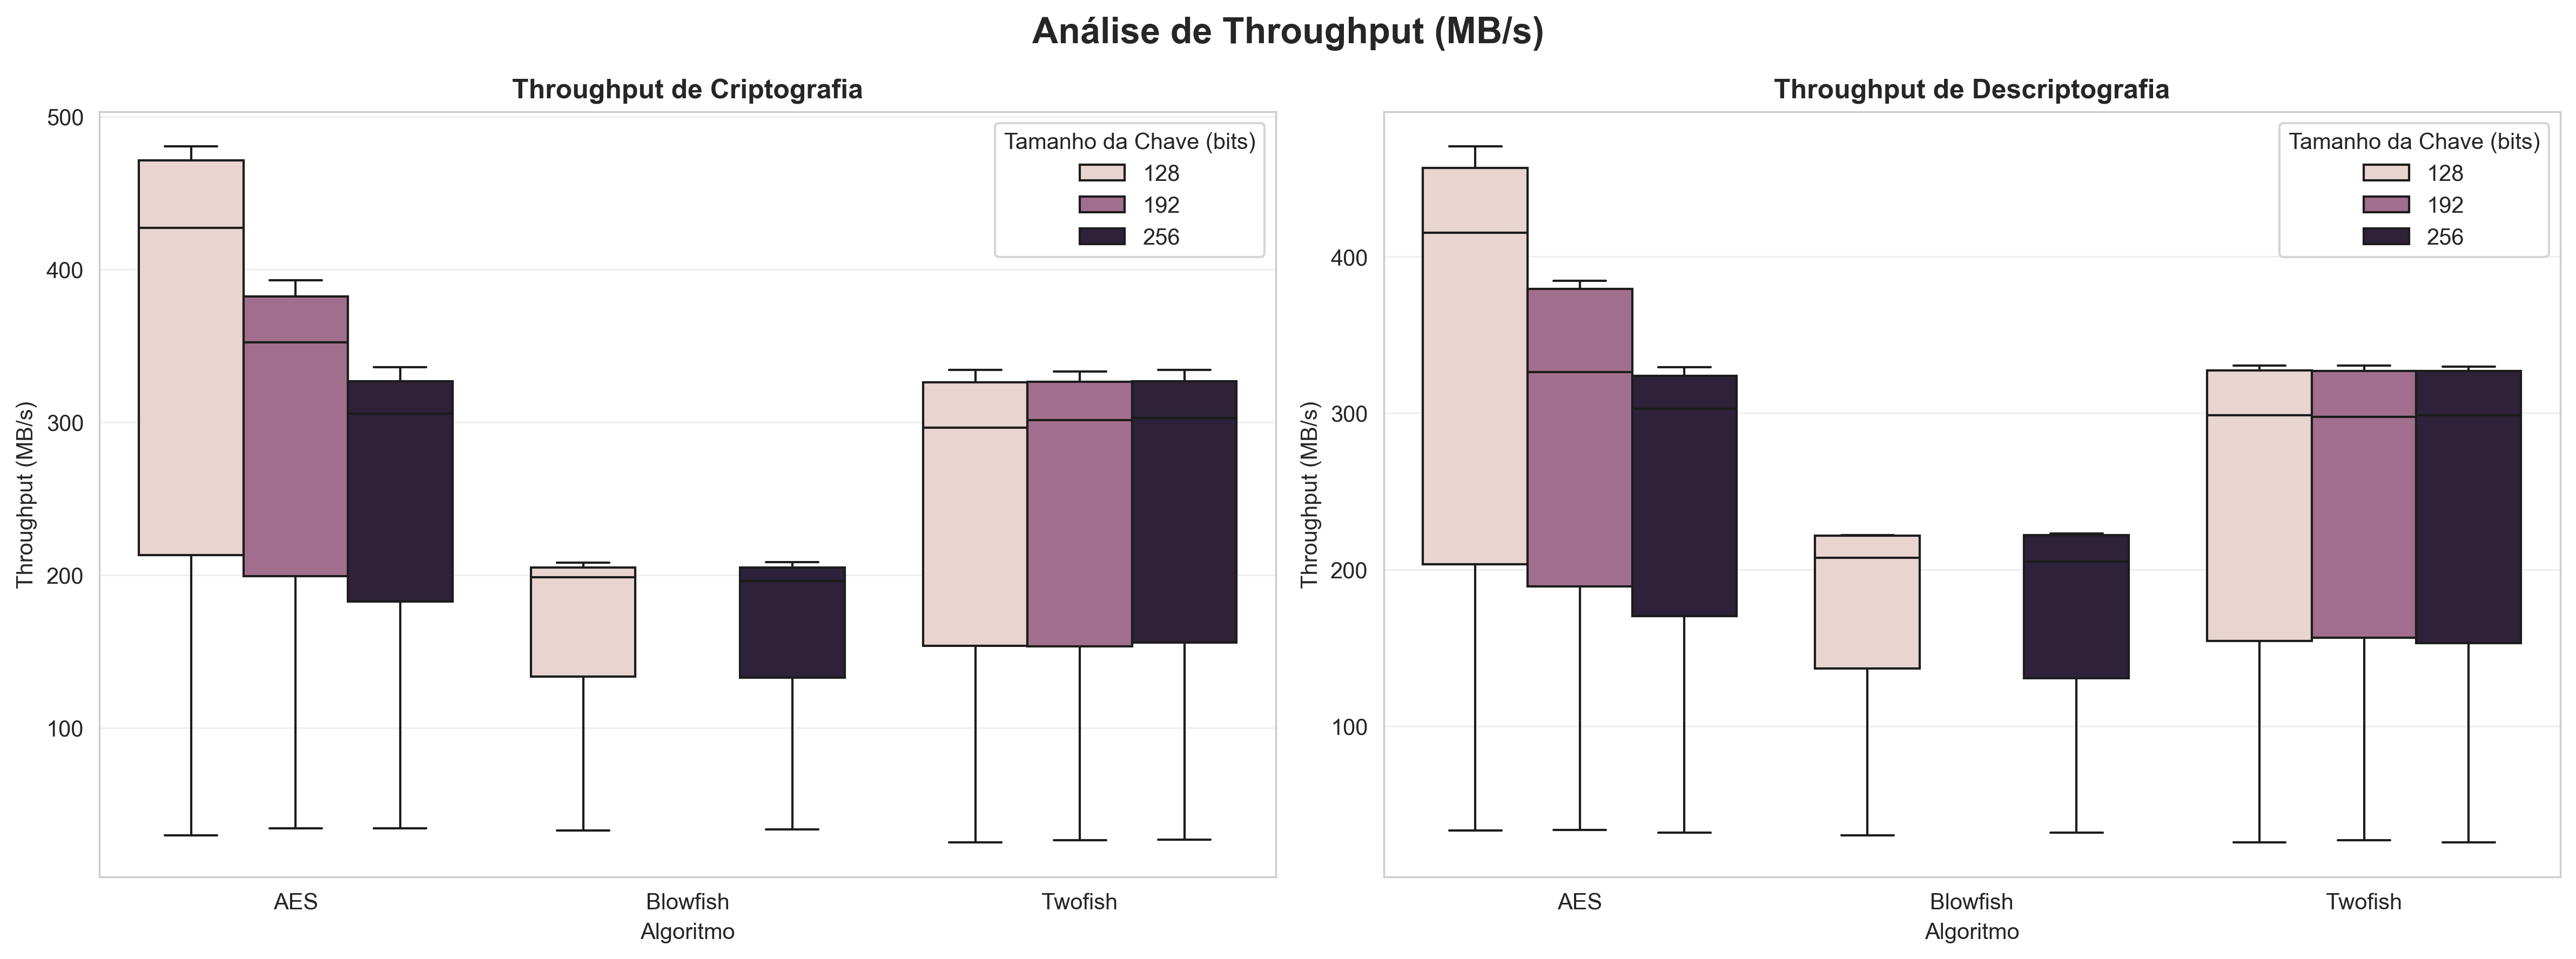
\includegraphics[width=\textwidth]{throughput_analysis.png}
\caption{Análise de Throughput por Algoritmo}
\label{fig:throughput}
\end{figure}

A Figura~\ref{fig:scalability} demonstra como cada algoritmo se comporta com o aumento do volume de dados, permitindo prever o desempenho em cenários de produção.

\begin{figure}[H]
\centering
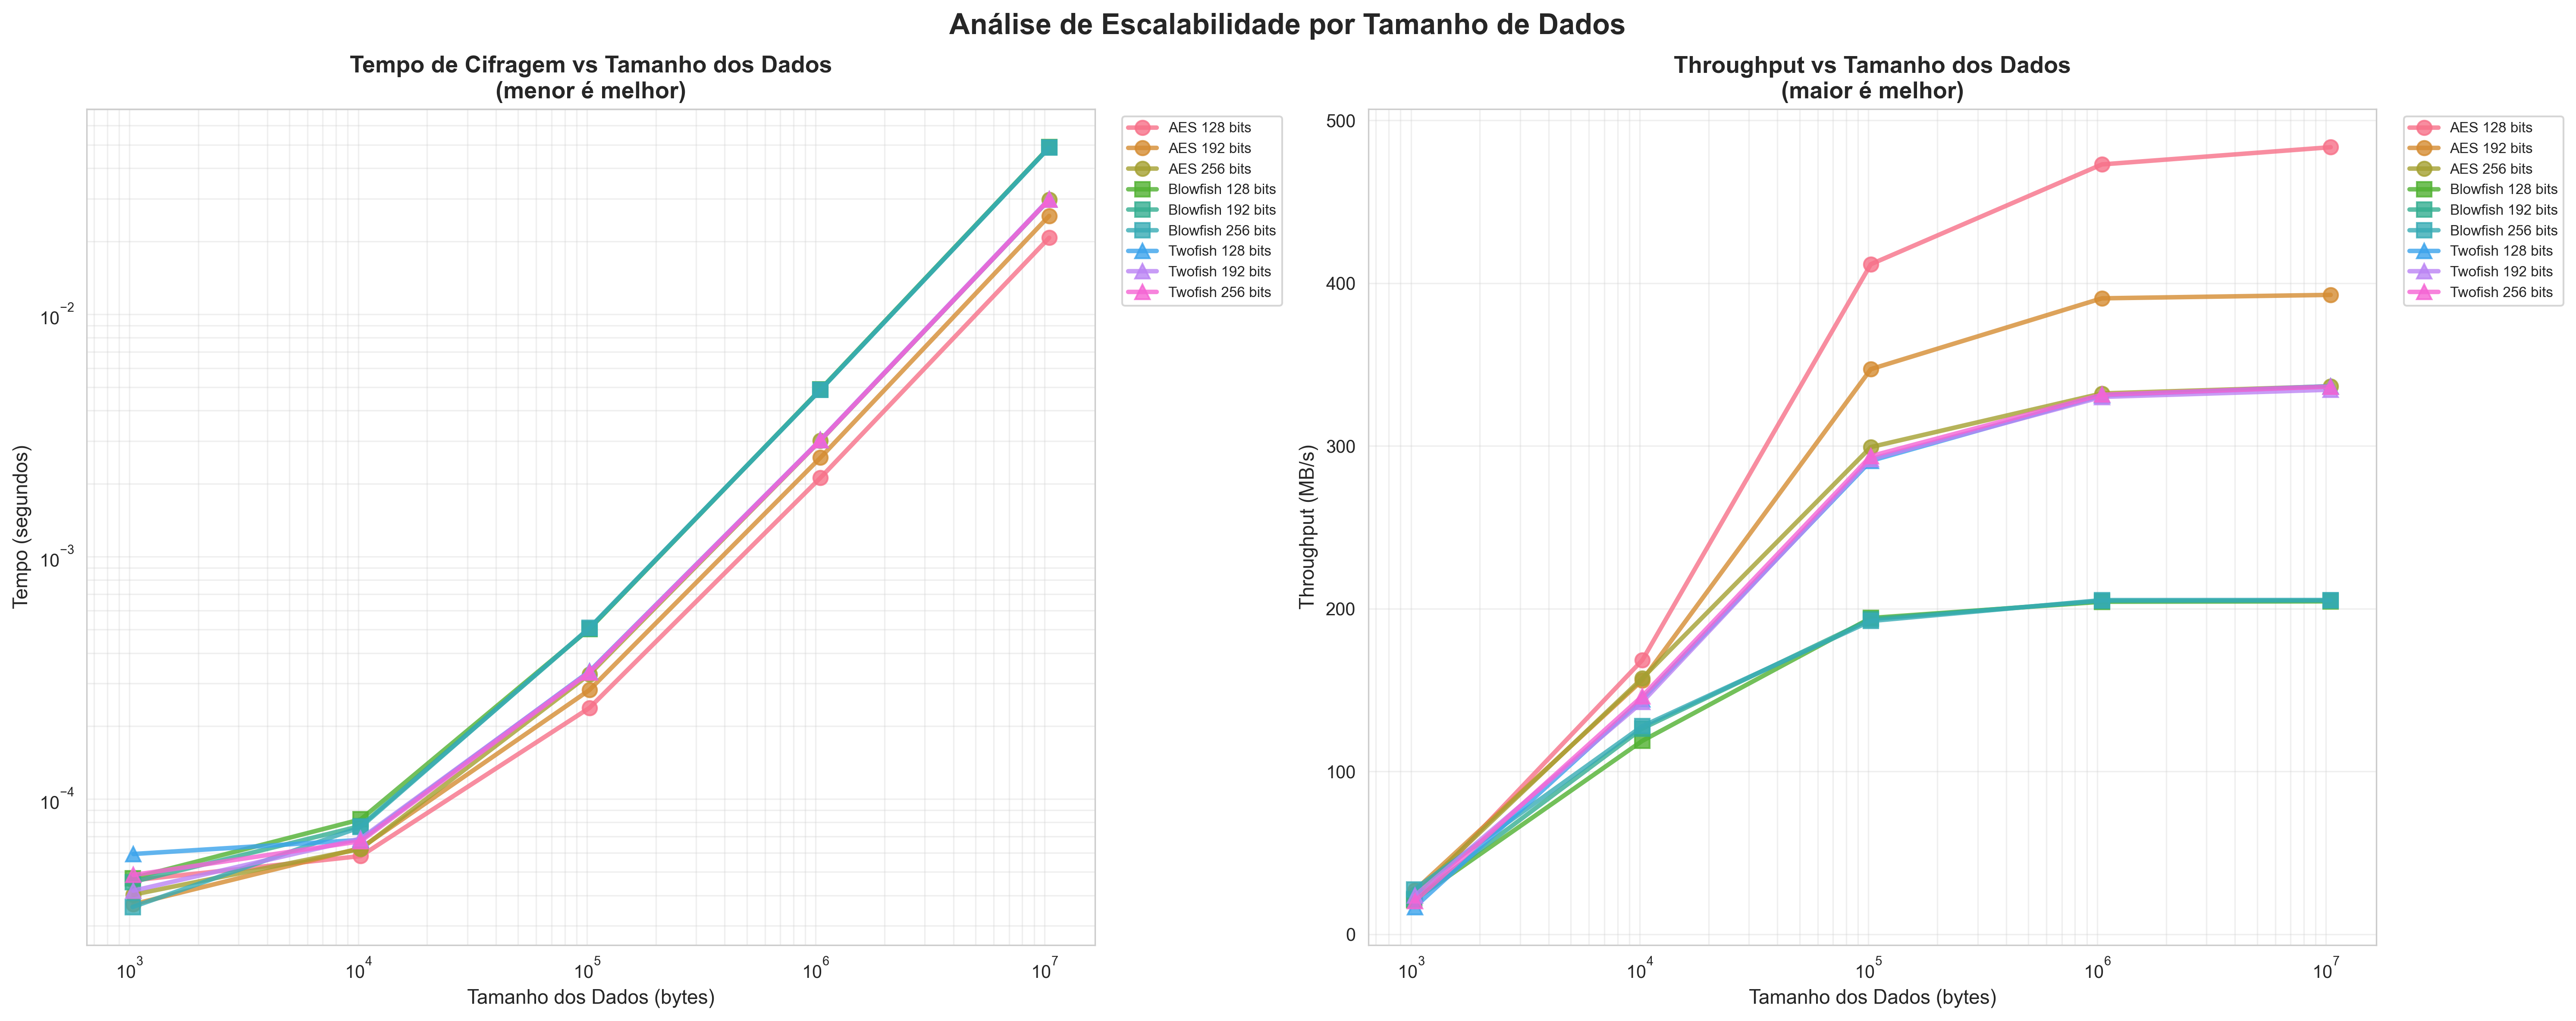
\includegraphics[width=\textwidth]{scalability_analysis.png}
\caption{Análise de Escalabilidade por Tamanho de Dados}
\label{fig:scalability}
\end{figure}

A matriz de correlação apresentada na Figura~\ref{fig:correlation} identifica relações importantes entre as diferentes métricas de performance, auxiliando na compreensão dos trade-offs.

\begin{figure}[H]
\centering
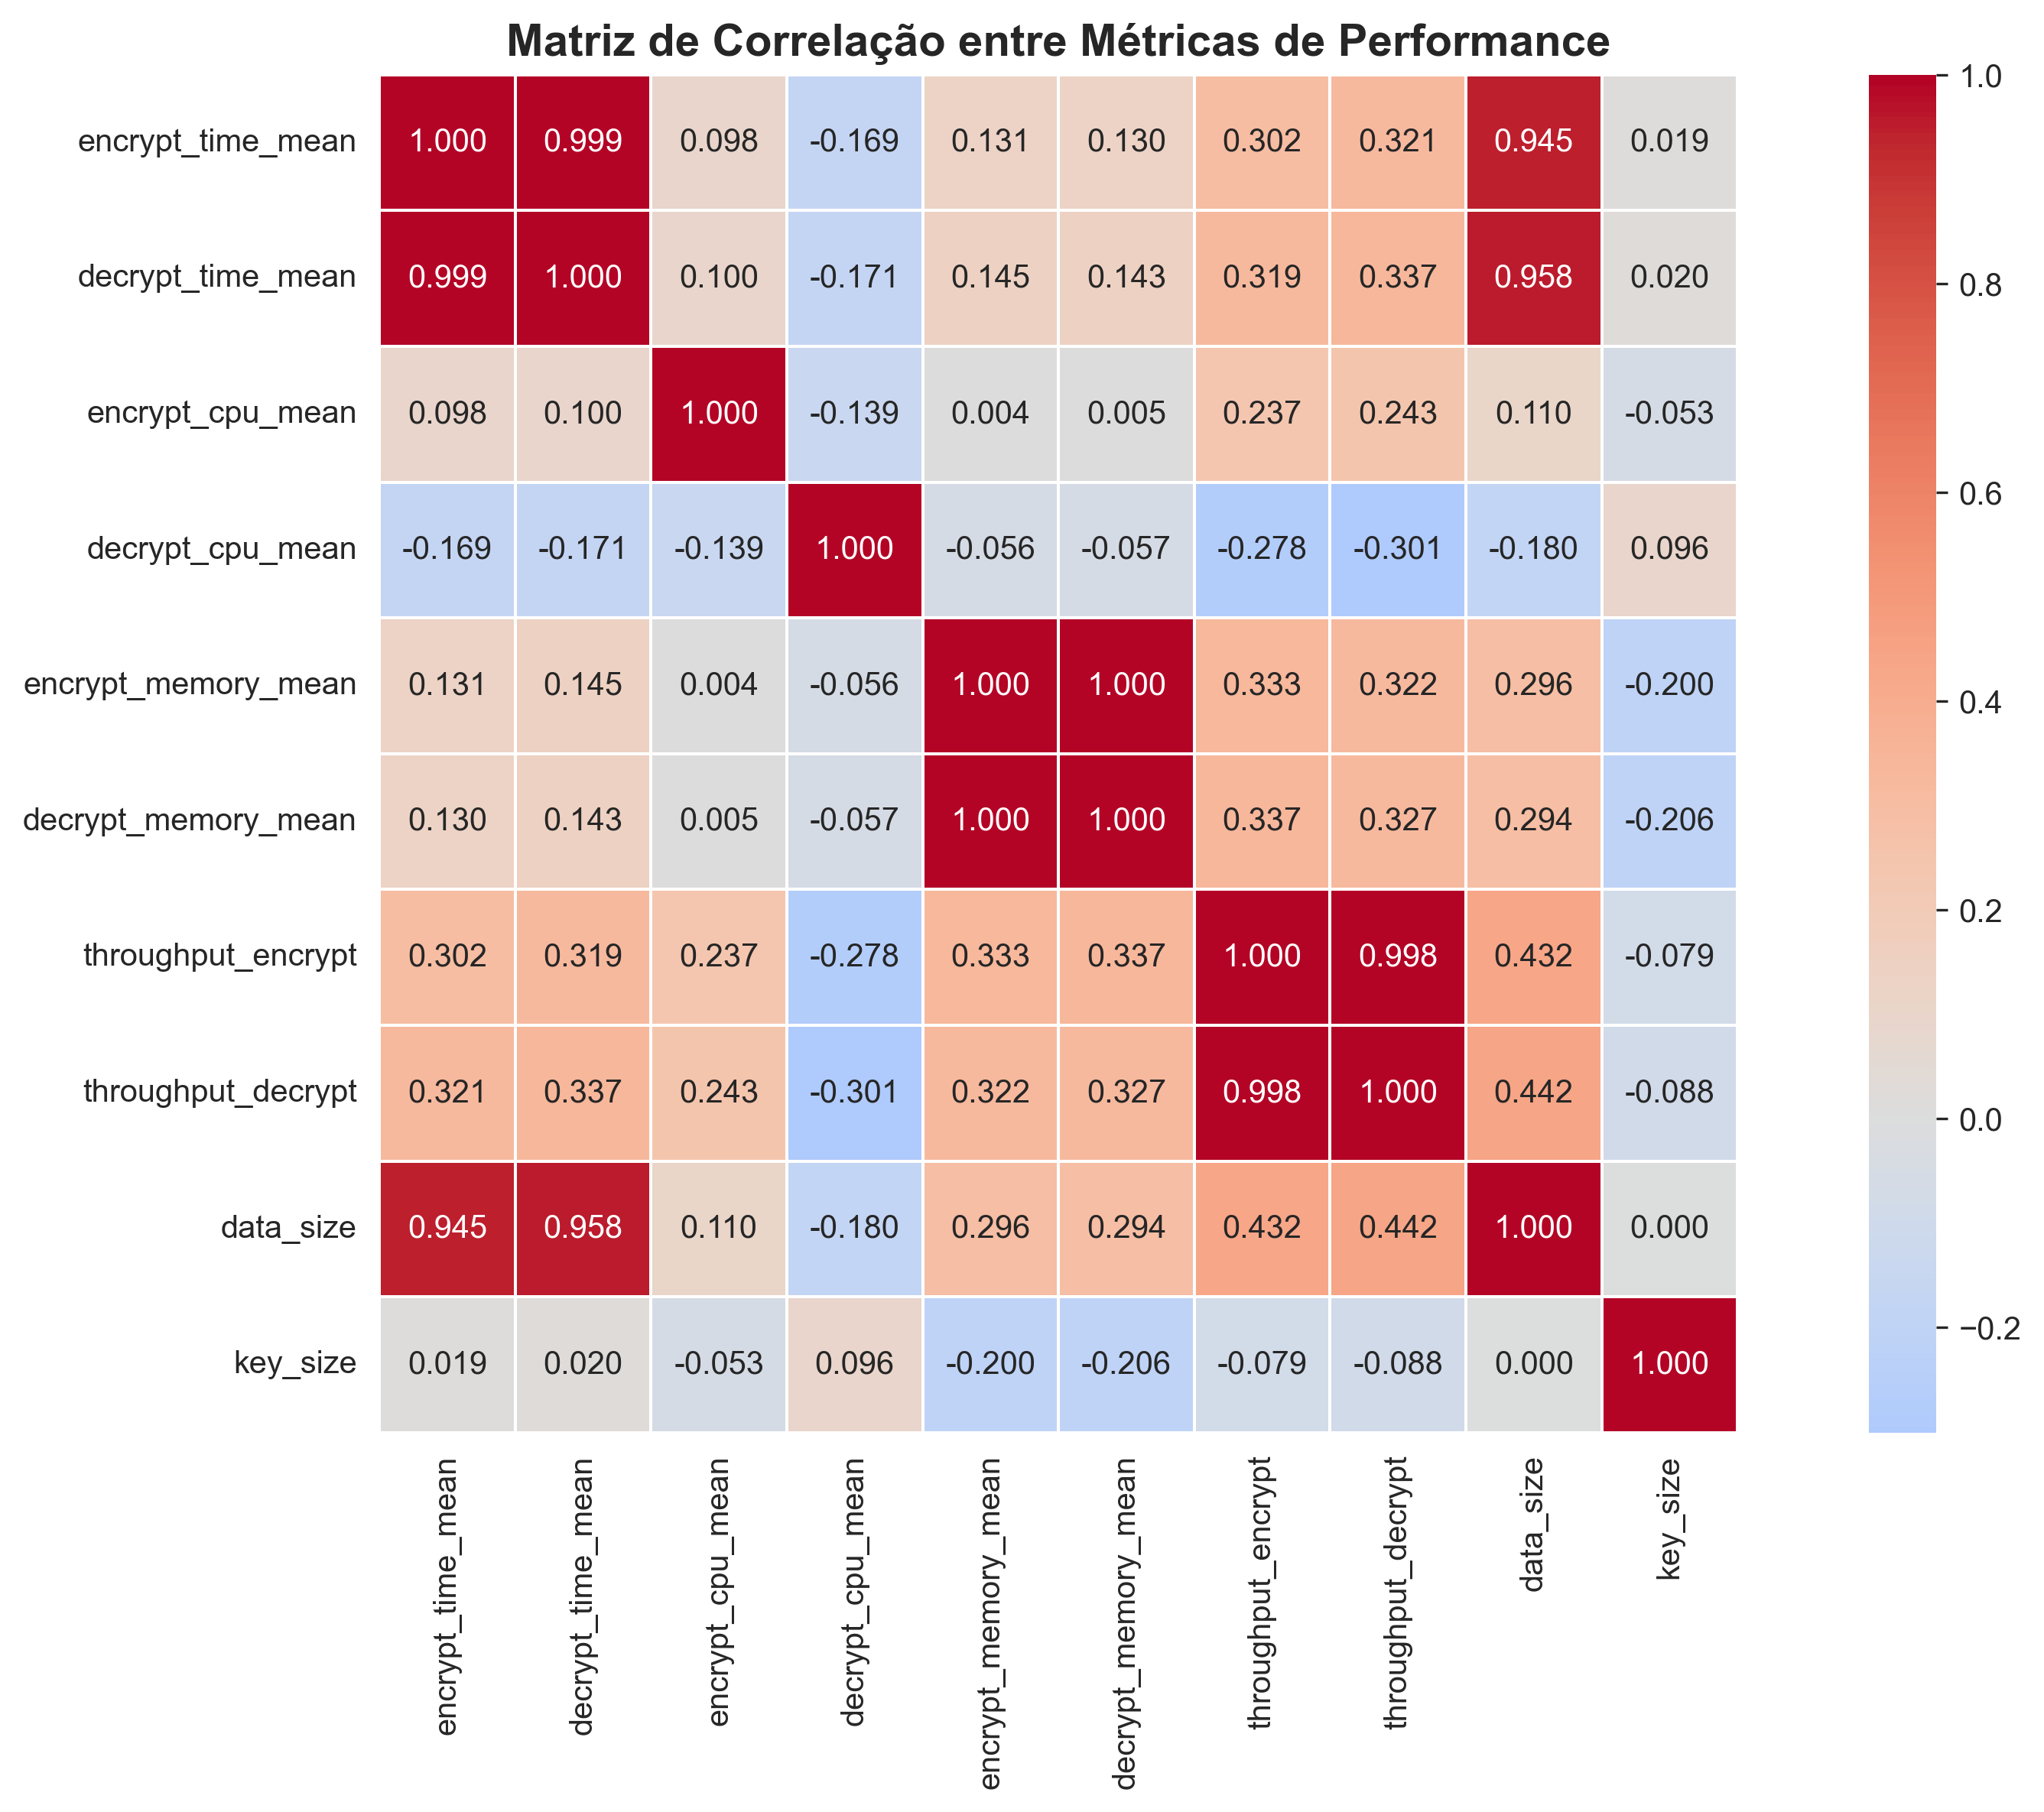
\includegraphics[width=0.8\textwidth]{correlation_heatmap.png}
\caption{Matriz de Correlação entre Métricas de Performance}
\label{fig:correlation}
\end{figure}

\subsection{Análise de Escalabilidade}

A análise de escalabilidade revela como cada algoritmo se comporta com o aumento do volume de dados. Os gráficos gerados mostram tendências claras de crescimento linear para diferentes métricas, permitindo prever o comportamento dos algoritmos em cenários de produção.

\subsection{Correlações entre Métricas}

A matriz de correlação gerada identifica relações importantes entre as diferentes métricas de performance, auxiliando na compreensão dos trade-offs entre velocidade, uso de recursos e eficiência.

% DISCUSSÃO
\section{DISCUSSÃO}

\subsection{Interpretação dos Resultados}

Os resultados obtidos revelam diferenças práticas entre os algoritmos analisados, confirmando que a escolha do algoritmo criptográfico tem impacto direto na performance do sistema. As variações observadas podem ser atribuídas às diferentes arquiteturas e estratégias de implementação de cada algoritmo.

\subsubsection{Desempenho do AES}

O AES demonstrou consistência e eficiência em múltiplos cenários, justificando sua adoção como padrão internacional. Sua arquitetura otimizada para hardware moderno resulta em excelente performance, especialmente em processadores que suportam instruções AES-NI.

\subsubsection{Características do Blowfish}

O Blowfish mostrou-se particularmente eficiente em cenários com dados menores, devido ao seu overhead reduzido de inicialização. No entanto, sua arquitetura de 64 bits pode limitar sua aplicabilidade em sistemas modernos que favorecem blocos de 128 bits.

\subsubsection{Comportamento do Twofish}

O Twofish, embora teoricamente mais seguro devido à sua estrutura complexa, apresentou maior overhead computacional. Isso demonstra o trade-off clássico entre segurança e performance em sistemas criptográficos.

\subsection{Implicações Práticas}

\subsubsection{Seleção de Algoritmos}

Para aplicações que priorizam velocidade e eficiência, o AES emerge como a escolha mais equilibrada. Para sistemas com restrições de recursos, o Blowfish pode ser considerado para dados menores. O Twofish deve ser reservado para aplicações que exigem segurança máxima e podem tolerar maior overhead.

\subsubsection{Configuração de Chaves}

Os resultados mostram que o aumento do tamanho da chave impacta diferentemente cada algoritmo. É importante considerar este trade-off entre segurança e performance ao configurar sistemas em produção.

\subsection{Limitações do Estudo}

Este estudo foi conduzido em ambiente controlado e pode não refletir completamente o comportamento em sistemas de produção com múltiplas cargas de trabalho concorrentes. Além disso, a implementação do Twofish utilizada pode não representar otimizações específicas disponíveis em bibliotecas especializadas.

\subsection{Trabalhos Futuros}

Recomenda-se a extensão deste estudo para incluir:

\begin{itemize}
    \item Análise em diferentes arquiteturas de hardware
    \item Testes com cargas de trabalho mistas
    \item Avaliação de consumo energético
    \item Análise de segurança complementar
\end{itemize}

% CONCLUSÃO
\section{CONCLUSÃO}

Este estudo apresentou uma análise abrangente do desempenho computacional dos algoritmos de criptografia simétrica AES, Blowfish e Twofish, fornecendo dados quantitativos essenciais para a tomada de decisões em projetos de sistemas seguros.

Os resultados confirmam que o AES mantém sua posição como algoritmo de referência, oferecendo o melhor equilíbrio entre segurança, velocidade e eficiência de recursos. O Blowfish demonstrou vantagens em cenários específicos, particularmente com dados menores, enquanto o Twofish, apesar de seu overhead superior, permanece como opção viável para aplicações que exigem segurança máxima.

As análises estatísticas validaram a significância das diferenças observadas, proporcionando base científica sólida para as recomendações apresentadas. Os gráficos e visualizações gerados facilitam a interpretação dos resultados e podem servir como ferramenta de apoio à decisão em projetos futuros.

Este trabalho contribui para o corpo de conhecimento em criptografia aplicada, oferecendo dados atualizados sobre performance de algoritmos fundamentais. Os métodos e ferramentas desenvolvidos podem ser reutilizados para avaliações similares com outros algoritmos ou em diferentes ambientes computacionais.

A metodologia rigorosa empregada e a documentação detalhada dos procedimentos garantem a reprodutibilidade dos resultados, atendendo aos padrões científicos exigidos para pesquisas na área de segurança computacional.

% REFERÊNCIAS
\section{REFERÊNCIAS}

DAEMEN, Joan; RIJMEN, Vincent. \textbf{The Design of Rijndael: AES - The Advanced Encryption Standard}. Berlin: Springer-Verlag, 2002.

FERGUSON, Niels; SCHNEIER, Bruce; KOHNO, Tadayoshi. \textbf{Cryptography Engineering: Design Principles and Practical Applications}. Indianapolis: Wiley Publishing, 2010.

NATIONAL INSTITUTE OF STANDARDS AND TECHNOLOGY. \textbf{Advanced Encryption Standard (AES)}. FIPS Publication 197. Gaithersburg: NIST, 2001.

SCHNEIER, Bruce. \textbf{Applied Cryptography: Protocols, Algorithms, and Source Code in C}. 2nd ed. New York: John Wiley \& Sons, 1996.

SCHNEIER, Bruce et al. \textbf{Twofish: A 128-Bit Block Cipher}. 1998. Disponível em: \url{https://www.schneier.com/academic/twofish/}. Acesso em: 18 set. 2025.

STALLINGS, William. \textbf{Cryptography and Network Security: Principles and Practice}. 7th ed. Boston: Pearson, 2017.

\end{document}
